\documentclass[11pt, a4paper]{article}

\usepackage{amsmath}
\usepackage{amsfonts}
\usepackage{graphicx}
\usepackage[export]{adjustbox}
\usepackage{hyperref}
\usepackage{fullpage}
\usepackage{caption}
\usepackage{listings}
\usepackage[dvipsnames]{xcolor}
\usepackage{gensymb}
\hypersetup{
    bookmarks=true,         % show bookmarks bar?
    unicode=false,          % non-Latin characters in Acrobat’s bookmarks
    pdftoolbar=true,        % show Acrobat’s toolbar?
    pdfmenubar=true,        % show Acrobat’s menu?
    pdffitwindow=false,     % window fit to page when opened
    pdfstartview={FitH},    % fits the width of the page to the window
    pdftitle={My title},    % title
    pdfauthor={Author},     % author
    pdfsubject={Subject},   % subject of the document
    pdfcreator={Creator},   % creator of the document
    pdfproducer={Producer}, % producer of the document
    pdfkeywords={keyword1, key2, key3}, % list of keywords
    pdfnewwindow=true,      % links in new PDF window
    colorlinks=true,       % false: boxed links; true: colored links
    linkcolor=Blue,          % color of internal links (change box color with linkbordercolor)
    citecolor=green,        % color of links to bibliography
    filecolor=magenta,      % color of file links
    urlcolor=red           % color of external links
}

\title{MAAS - Project Report \\Commitment Issues}
\author{Sushant Vijay Chavan\\Ahmed Faisal Abdelrahman\\Abanoub Abdelmalak}
\date{\today}

\begin{document}
\maketitle
\newpage
\tableofcontents{}
\newpage

\section{Introduction}
This project was completed as a part of the project work for the Multi-Agent and Agent Systems course. In this project we implemented two stages (Packaging and Delivery) of the Flying Saucers Bakery project. In addition we implemented visualization of the delivery stage as a street network with moving trucks to show the delivery in action. 

\textbf{TODO}

\section{Packaging Stage}\label{PackagingStage}
\paragraph{}
This stage deals with completion of the post baking stages and then packaging the products into boxes so that they are ready for delivery. The stage receives the baked and cooled products from the cooling racks and preforms the final preparation of the products such as sprinkling and decorating according to the recipe for the product. Once the products are ready, they are packed into boxes based on the delivery date priority of the orders. Once all the boxes of a given product type in an order are ready, they are sent to the delivery stage for transportation.

\paragraph{}
Figure \ref{PackagingArchitecture} gives an overview of the architecture of the packaging stage. This stage consists of three agents and in addition communicates with the CoolingRacks agent to receive the cooled products. The GenericItemProcessor takes care of all the post-baking steps, where as the packaging agent boxes the products based on the order priority. The Loading bay keeps track of the produced quantity of the products and informs the delivery stage whenever all products of a type in an order are ready.

\begin{figure}[h!]
	\centering
	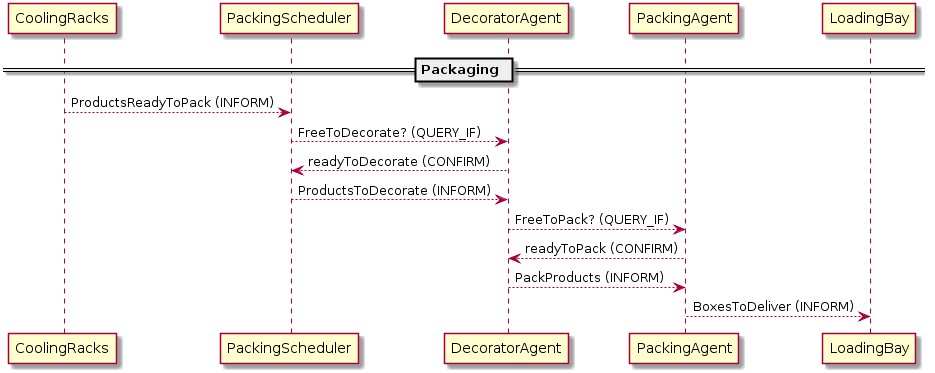
\includegraphics[width=\textwidth]{../Architecture/Architecture_Packaging.png}
	\caption{Packaging Stage Architecture}
	\label{PackagingArchitecture}
\end{figure}

\paragraph{}
The output of this stage is a set of boxes that consists of a fulfilled item from a customer order. For example, if a customer order consists of 10 breads and 15 donuts, assuming that the loading bay sees that the 15 donuts of this order are available, it sends these boxes to the delivery stage. Please note that not all products of this order are yet complete and that the loading bay will wait until all the breads of this order are available before sending out a new message to the delivery stage.

\subsection{Agents}\label{PackagingAgents}
\begin{enumerate}
	\item \textit{Generic Item Processor} (Owner: Abanoub):\\
	Description
	\item \textit{Packaging agent} (Owner: Sushant):\\
	This agent is responsible for receiving the ready products and then packaging them into boxes. The packaged boxes are then sent to the loading bay so that they can be dispatched to the customer. This agent prioritizes the packaging of the received products based on the delivery time of the orders. For example, assume we have two orders requiring 10 and 20 breads respectively and that the delivery date of the first order is earlier than that of the second. Now if we receive 20 breads from the previous stage, the packaging agents first boxes the 10 breads for the first order and sends them to the LoadingBay. It then packages the remaining 10 breads as a part of the second order. It must be noted that the packaging agent sends out the boxes as soon as they are full. It expects the loading bay to store the boxes until an all boxes of a product in an order are ready.
	\item \textit{Loading Bay} (Owner: Ahmed):\\
	Description and message description
\end{enumerate}

\newpage
\section{Delivery Stage}\label{DeliveryStage}
\paragraph{}
This stage handles the delivery of the packaged boxes from the bakery to the customers. The inputs to this stage are a set of boxes from the packaging stage as described in the section \ref{PackagingStage}. This stage waits until all the products of an order are ready for dispatch and then requests the trucks for transportation of these boxes. Once the orders have been delivered to the customer, the trucks post the status of the delivery to the mailbox, which then informs all agents that are interested in this information.

\paragraph{}
This stage consists of 5 agents as shown the architecture diagram in figure \ref{DeliveryArchitecture}. In addition this stage talks with two other agents: \textit{LoadingBayAgent} and the \textit{GraphVisualizationAgent}. The figure gives an overview of the communication happening between the agents in order to complete an order received from the LoadingBayAgent. The visualization of the delivery stage will be explained in detail in section \ref{GraphVisualizationAgent}. However it is helpful to know that the only agents that need to communicate with the GraphVisualizationAgent are the StreetNetworkAgent and the TruckAgents. 

\begin{figure}[h!]
	\centering
	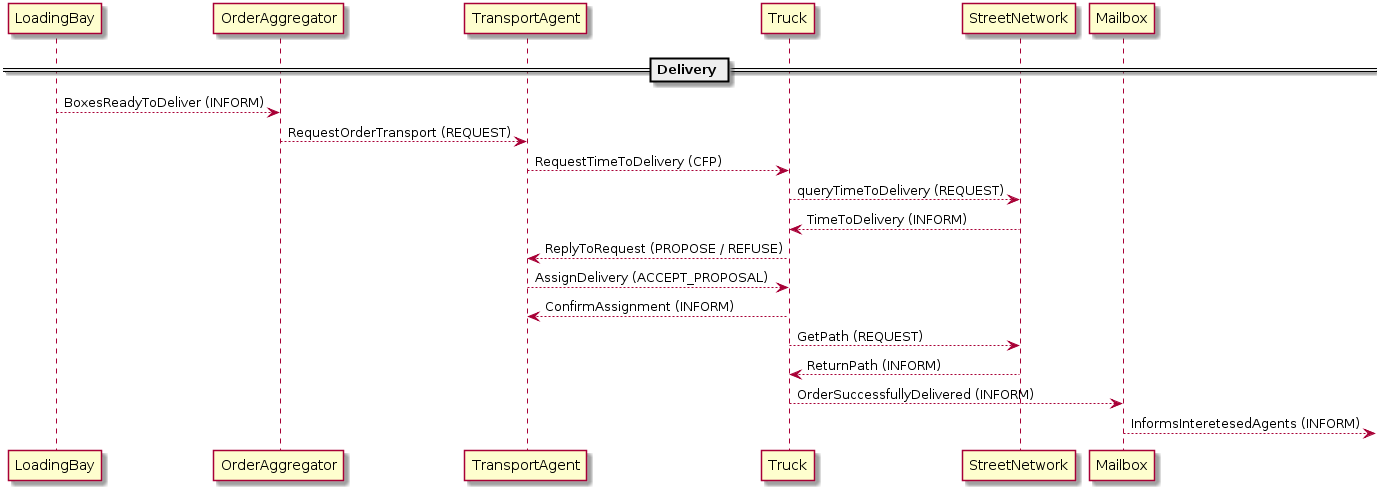
\includegraphics[width=\textwidth]{../Architecture/Architecture_Delivery.png}
	\caption{Delivery Stage Architecture}
	\label{DeliveryArchitecture}
\end{figure}

\paragraph{}
In order to find the best truck that can deliver the orders, the transport agent of the bakery requests for proposals from the trucks to deliver the order. Each Truck which is capable of delivery this order then queries the StreetNetwork to find the time needed by it to complete its current task and then return to the bakery to collect the products and then move towards the customer. These estimates are then sent back to the transport agent, which then chooses that truck that has the least time to delivery.  Section \ref{DeliveryAgents} provides a detailed description of all the agents that are a part of the delivery stage.

\subsection{Agents}\label{DeliveryAgents}
\begin{enumerate}
	\item \textit{OrderAggregator} (Owner: Abanoub):\\
	Description
	\item \textit{TransportAgent} (Owner: Abanoub):\\
	Description
	\item \textit{TruckAgent} (Owner: Sushant):\\
	This agent is responsible for collecting orders from a bakery and delivering them to the customers. Each truck is associated with a transport company and multiple transport companies could exist. It is responsible for querying the estimated delivery time for an order and proposing this to the transport agent. If the proposal is accepted, it is also responsible for moving towards the bakery to collect the orders and the move towards the customers to deliver them. Finally it also informs the status of the delivery (such as the time of delivery, number of boxes) to the mailbox. Due to its highly dynamic nature, this agent has an extensive communication with other agents, as can be seen from the figure \ref{DeliveryArchitecture}. It must be noted that with the current implementation, every truck can accept atmost one extra order in addition to the one it is currently handling. 
	
	Additionally this agent also communicates with the GraphVisualizationAgent in order to send its position and status updates for visualization. 
	\item \textit{StreetNetworkAgent} (Owner: Ahmed):\\
	Description
	\item \textit{Mailbox} (Owner: Ahmed):\\
	Description and message description
\end{enumerate}

\newpage
\subsection{Graph Visualization Agent}\label{GraphVisualizationAgent}
Screenshot of the graph along with short description. Add reference to the codes source. 
\\Owners: All

\begin{figure}[h!]
	\centering
	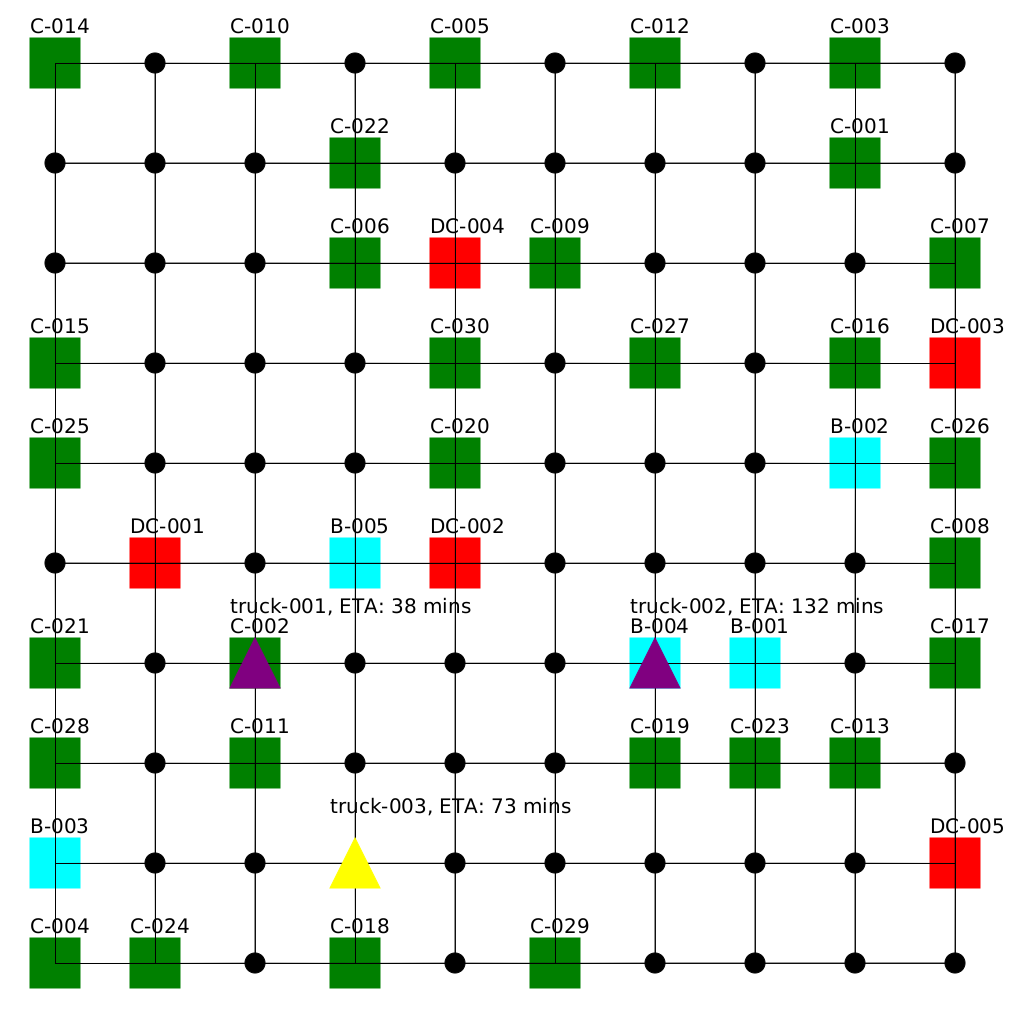
\includegraphics[width=\textwidth]{Visualization.png}
	\caption{Visualization Screenshot}
	\label{PackagingArchitecture}
\end{figure}

\newpage
\section{Entry Agent}
Owner: Sushant
\paragraph{}
In order to test the two developed stages independent of the other stages, we need an agent that can trigger the first agent of the cooling racks agent to start the simulation. The EntryAgents fulfills this requirement. Using this agent, it is possible to simulate that the products from of an order have been baked and are ready for cooling, which then starts the two following stages until the order has been delivered to the customer. It should be noted that the EntryAgent simply uses the order information available in the scenario files and does not generate any data on its own.

\paragraph{}
The Entry agent has two functionalities. First, it reads the order details from the currently active scenario directory and then generates dummy messages that inform the cooling rack that the products of an order are ready. These messages are then sent to the cooling rack at the delivery time mentioned in the scenario file. Therefore the first part of this agent acts as the trigger for the two stages. Since the order processor agent was also not available on the upstream repository, we added the order processor functionality as the second functionality of the entry agent. Whenever an order is sent to the cooling rack, a corresponding order information is also broadcasted to all agents. We used the same  message format as the actual order processor. This way we ensure that all our agents are compatible with the actual order processor, whenever it is available.

\section{Usage Instructions}

\subsection{Running the two stages}

\subsection{Running on distributed systems}

\section{Conclusion}

\end{document}\grid
